% ---- ETD Document Class and Useful Packages ---- %
\documentclass{ucetd}
\usepackage{subfigure,epsfig,amsfonts}
\usepackage{natbib}
\usepackage{amsmath}
\usepackage{amssymb}
\usepackage{amsthm}
\usepackage[toc,page]{appendix}
\usepackage[labelfont=bf]{caption}
\usepackage{rotating}
\usepackage[dvipsnames]{xcolor}
\usepackage{url}
\usepackage{bm}
\usepackage{bbm}

%% Use these commands to set biographic information for the title page:
\title{Visualizing nucleosome cluster dynamics with dense single molecule localization microscopy}
\author{Clayton W. Seitz}
\department{Department of Physics}
\division{Physical Sciences}
\degree{Doctor of Philosophy}
\date{Spring 20XX}

%% Use these commands to set a dedication and epigraph text

\epigraph{Epigraph}



\begin{document}
%% Basic setup commands
% If you don't want a title page comment out the next line and uncomment the line after it:
\maketitle
%\omittitle

% These lines can be commented out to disable the copyright/dedication/epigraph pages
\makecopyright
%\makededication


%% Make the various tables of contents
\tableofcontents
%\listoffigures
%\listoftables

%\acknowledgments
% Enter Acknowledgements here

\abstract

Single-molecule localization-based super-resolution microscopy techniques, such as direct stochastic optical reconstruction microscopy (dSTORM), can be used to produce a pointillist representation of nucleosome organization at diffraction-unlimited precision. Direct STORM approaches leverage the deactivation of fluorescent tags, followed by spontaneous or photoinduced reactivation, to achieve super-resolution reconstructions of nuclear proteins and nucleic acids. This basic principle remains one of the method's primary limitations - standard analysis algorithms require tight control of activation and reactivation to maintain sparse emitters, presenting a tradeoff between imaging speed and labeling density. Here, we present a dSTORM strategy for fast reconstruction of nucleosome organization in living cells by complementing high duty-cycle blinking of rhodamine-derived dyes with a novel localization algorithm based on deep generative modeling. Previous approaches to breaking the time resolution barrier in SMLM learn prior information about cellular structures using generative models and predict super-resolution images based on sparse localizations, or interpolate and transform dense images into a localization map. However, cellular structures such as chromatin are dynamic and intrinsically heterogeneous; therefore, structures cannot necessarily be known apriori. Furthermore, localization maps are parametric and non-probabilistic, making them highly application specific, and difficult to use. We propose an alternative method based on directly modeling the distribution of high resolution images conditioned on a low resolution image. By performing high density localization, we can directly visualize 1,6 Hexanediol induced chromatin reorganization over minute time scales.


\clearpage

\mainmatter

\chapter{}

\section{Introduction}

Single molecule localization microscopy (SMLM) relies on the temporal resolution of fluorophores in the sample whose spatially overlapping point spread functions would otherwise render them unresolvable at the detector. SMLM techniques, such as stochastic optical reconstruction microsscopy (STORM) and photoactivatable localization microscopy (PALM) remain desirable for super-resolution imaging of many cellular structures, due to their cost-effective implementation and photon-count limited resolution (Schermelleh 2019). Common strategies for the temporal separation of molecules involve transient intramolecular rearrangements to switch from dark to fluorescent states or the exploitation of non-emitting molecular radicals. Reduced rhodamine derivates in particular can be quenched by oxidative processes or form dark radical species, which absorb strongly around 400 nm, a property that can be exploited to drive the fluorophore back to its ground state. Long dark state lifetimes are commonly used in STORM imaging, while quenching results in a higher duty cycle and increased rates of photobleaching due to irreversible oxidative damage of important functional groups. Nevertheless, high duty cycle SMLM can greatly reduce acquisition times and increase labeling density while permitting the recording of some dynamic processes (Speiser 2021). Fluorescent labeling density has been known to pose a major bottleneck to super-resolution imaging acqusitions. Static uncertainty due to molecular crowding can be partially amelioriated by using pairwise or higher-order temporal correlations within a pixel neighborhood, known as stochastic optical fluctuation imaging (Dertinger 2009). Other approaches such as stimulated emission and depletion (STED) imaging bring control over the photophysical state of a chosen subset of the sample, yet the need for laser scanning prevents widespread application in live-cell studies. Therefore, in certain applications, the spatial resolution and paralellism of SMLM techniques remain unparalleled.


\subsection{Photoswitchable rhodamine derivatives for super-resolution microscopy}


\begin{figure}
\begin{center}
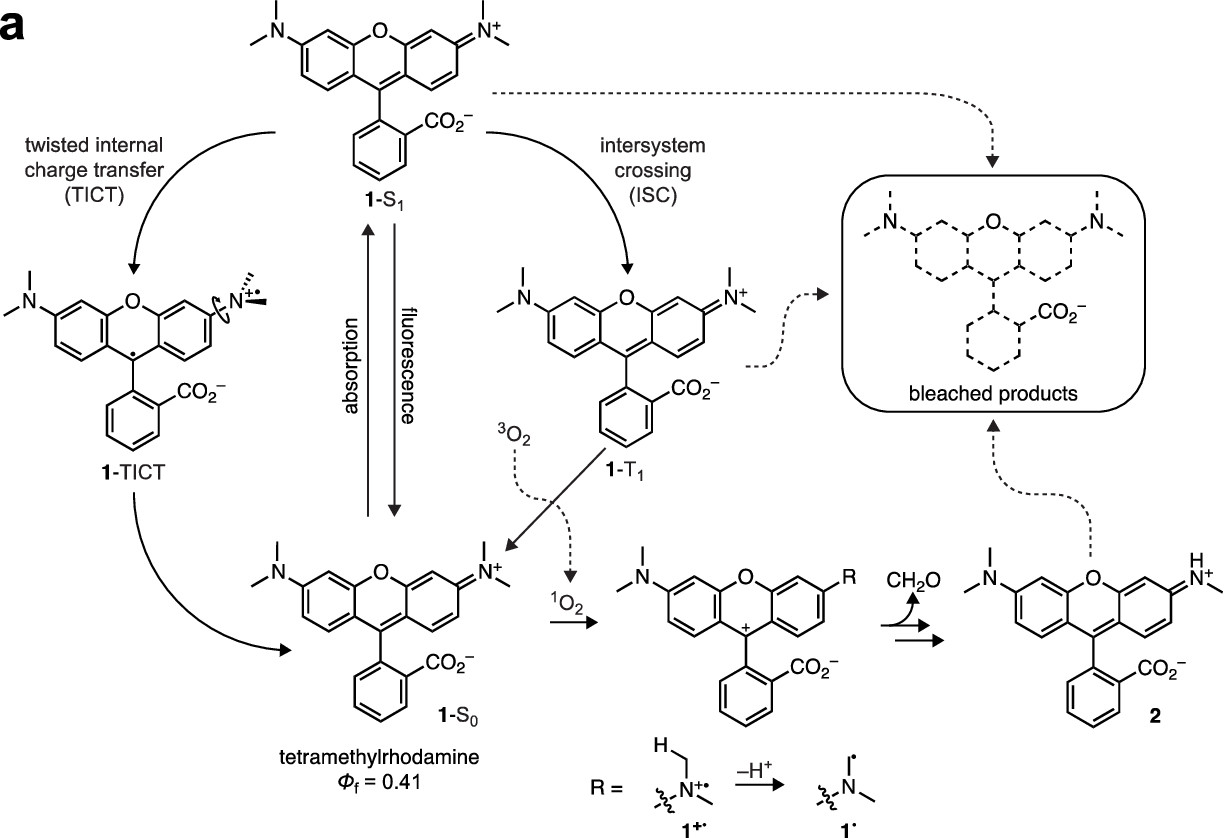
\includegraphics[width=14cm]{Rhodamines.png}
\end{center}
\end{figure}




\subsection{Estimator precision sets the resolution limit in localization microscopy}

Complementary Metal-Oxide-Semiconductor (CMOS) cameras have noise sources intrinsic to their operation, such as shot noise and readout noise. The former phenomenon can describe a superposition of processes; namely, the fluctuations of the number of photons due to the quantum nature of light, and the random conversion of photons into photoelectrons within the semiconductor material with a quantum efficiency below unity. Here we will often refer to the photon count $N_{0}$, which has a determined value, rather than being described by statistically. The \emph{measured} photon count, however, is well-described by a Poisson process as variance of counts is equal to the mean (Schottky 1918). A shot-noise limited image is then described as a family of Poisson variables, with units of photoelectrons

\begin{figure}
\begin{center}
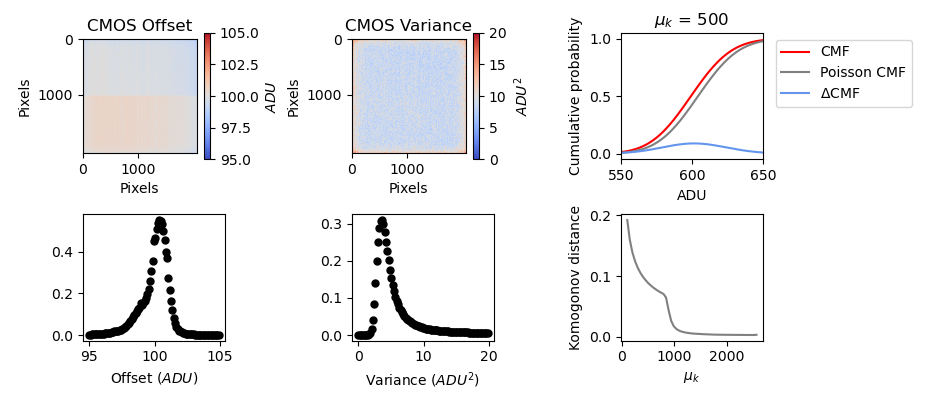
\includegraphics[width=16cm]{Noise.png}
\end{center}
\end{figure}




\begin{equation}
\vec{S} = \left[\mathrm{Poisson}(\mu_{1}), \mathrm{Poisson}(\mu_{2}), ..., \mathrm{Poisson}(\mu_{N})\right]
\end{equation}

Since CMOS sensors also suffer from other noise sources, which may refer to so-called readout noise or dark current, there can be a nonzero signal even in the absence of incident light. Dark current is due to statistical fluctuations in the photoelectron count within a semiconductor material in thermal equilibrium. Fortunately, these additional noise sources are governed by the central limit theorem, and can be efficiently summarized as the component of the noise which exhibits a Gaussian distribution. Readout noise has been often neglected in localization algorithms because its presence in EMCCD cameras is small enough that it can be ignored within the tolerances of the localization precision. In the case of high speed sCMOS cameras, however, the readout noise of each pixel is significantly higher and, in addition, every pixel has its own noise and gain characteristic sometimes with dramatic pixel-to-pixel variations. The number of photoelectrons $S_{k}$ is  multiplied by a gain factor $g_{k}$ which has units of $[\mathrm{ADU}/e^{-}]$, which generally must be measured for each pixel. Here, we will always assume that readout noise per pixel $\xi_{k}$ is Gaussian with some pixel-specific offset $o_{k}$ and variance $\sigma_{k}^{2}$. Ultimately, we have a Poisson component of the noise, which scales with the signal level and a Gaussian component, which does not. Therefore, our measurement is: 

\begin{equation}
\vec{H} = \vec{S} + \vec{\xi}
\end{equation}

What we are after is the joint distribution $P(\vec{H})$. A fundamental result in probability theory is that the distribution of $H_{k}$ is the convolution of the distributions of $S_{k}$ and $\xi_{k}$,

\begin{align}
P(H_{k}|\theta) &= P(S_{k})\circledast P(\xi_{k})\\
&= A\sum_{q=0}^{\infty} \frac{1}{q!}e^{-\mu_{k}}\mu_{k}^{q}\frac{1}{\sqrt{2\pi}\sigma_{k}}e^{-\frac{(H_{k}-g_{k}q-o_{k})}{2\sigma_{k}^{2}}}
\end{align}

where $P(\xi_{k}) = \mathcal{N}(o_{k},\sigma_{k}^{2})$ and $P(S_{k}) = \mathrm{Poisson}(g_{k}\mu_{k})$. In practice, this expression is difficult to work with, so we look for an approximation. Notice that 

\begin{align*}
\xi_{k} - o_{k} + \sigma_{k}^{2} \sim \mathcal{N}(\sigma_{k}^{2},\sigma_{k}^{2}) \approx \mathrm{Poisson}(\sigma_{k}^{2})
\end{align*}

Since $H_{k} = S_{k} + \xi_{k}$, we transform $H_{k}' = H_{k} - o_{k} + \sigma_{k}^{2}$, which is distributed according to 

\begin{align*}
H_{k}' \sim \mathrm{Poisson}(\mu_{k}')
\end{align*}

where $\mu_{k}' = g_{k}\mu_{k} + \sigma_{k}^{2}$. This result can be seen from the fact the the convolution of two Poisson distributions is also Poisson.

\subsubsection{Integrated isotropic Gaussian point spread function}

Due to diffraction, any point emitter, such as a single fluorescent molecule, will appear at the image plane as a diffraction limited spot. For the sake of simplicity, it is common to describe the point spread function as a two-dimensional isotropic Gaussian (Zhang 2007):

\begin{equation*}
\mathrm{G}(x,y) = \frac{1}{2\pi\sigma^{2}}e^{-\frac{(x-x_{0})^{2}+(y-y_{0})^{2}}{2\sigma^{2}}}
\end{equation*}

The image of a fluorescent molecule capture by the objective lens, can be thought of as two-dimensional histogram of photon arrivals and a discretized form of the classical intensity profile $\mathrm{G}(x,y)$. The value at a pixel approaches an integral of this density over the pixel:

\begin{equation}
\mu_{k} = i_{0}\lambda_{k} = i_{0}\int_{\mathrm{pixel}} G(x,y)dxdy
\end{equation}

Let $(x_{k},y_{k})$ be the center of pixel $k$. If a fluorescent molecule is located at $(x_{0},y_{0})$, the probability of a photon arriving at pixel $k$ per unit time reads

\begin{equation*}
\lambda_{k} = \int_{x_{k}-\frac{1}{2}}^{x_{k}+\frac{1}{2}}G(x-x_{0})dx \int_{y_{k}-\frac{1}{2}}^{y_{k}+\frac{1}{2}} G(y-y_{0})dy
\end{equation*}

\vspace{0.2in}
where $i_{0} = g_{k}\eta N_{0}\Delta$. The parameter $\eta$ is the quantum efficiency and $\Delta$ is the exposure time. $N_{0}$ represents the number of photons emitted per unit time. We can then express the Gaussian integrals over a pixel by making use of the following property of the error function

\begin{equation*}
\frac{1}{\sqrt{2\pi}\sigma}\int_{a}^{b} e^{\frac{-(x-\mu)^{2}}{2\sigma^{2}}} = \frac{1}{2}\left(\mathrm{erf}\left(\frac{b-\mu}{\sqrt{2}\sigma}\right) -\mathrm{erf}\left(\frac{a-\mu}{\sqrt{2}\sigma}\right)\right)
\end{equation*}

This gives a convenient expression for the fraction of photons which arrive at a pixel $k$

\begin{align*}
\lambda_{k}(x) &= \frac{1}{2}\left(\mathrm{erf}\left(\frac{x_{k}+\frac{1}{2}-x_{0}}{\sqrt{2}\sigma}\right) -\mathrm{erf}\left(\frac{x_{k}-\frac{1}{2}-x_{0}}{\sqrt{2}\sigma}\right)\right)\\
\lambda_{k}(y) &= \frac{1}{2}\left(\mathrm{erf}\left(\frac{y_{k}+\frac{1}{2}-y_{0}}{\sqrt{2}\sigma}\right) -\mathrm{erf}\left(\frac{y_{k}-\frac{1}{2}-y_{0}}{\sqrt{2}\sigma}\right)\right)
\end{align*}

\subsubsection{Integrated astigmatic Gaussian point spread function}

In order to generalize our model to three-dimensions, we could use that the isotropic Gaussian point spread function has a variance which is dependent on the axial coordinate (Figure 3B). However, it has been shown that the error around the focus can be large, while negative and positive defocus cannot be distinguished given the symmetric dependence in $z$ (Holtzer 2007). Therefore, for 3D microscopy, a rather simple approach is to introduce astigmatism into the detection path using a weak cylindrical lens (Huang 2008). In effect, this breaks the axial symmetry of the PSF and gives an anisotropic Gaussian which is elongated perpendicular to the optical axis. Localization proceeds by measuring this anisotropy and inverting a model of its axial dependence. This axial anisotropy can be complex, but is often well described by a polynomial function of the axial displacement $z_{0}$

\begin{equation*}
\sigma_{x}(z_{0}) = \sum_{n}a_{n}z_{0}^{n}\;\;\;\; \sigma_{y}(z_{0}) = \sum_{n}b_{n}z_{0}^{n}
\end{equation*}

with the following continuous density over the pixel array

\begin{equation}
\mathrm{G}(x,y) = \frac{1}{2\pi\sigma_{x}(z)\sigma_{y}(z)}e^{-\frac{(x-x_{0})^{2}}{2\sigma_{x}(z_{0})^{2}}+\frac{(y-y_{0})^{2}}{2\sigma_{y}(z_{0})^{2}}}
\end{equation}


\subsubsection{Localization microscopy as frequentist inference}

According to our image formation, molecules really do have an exact location in space. In pratice, this is only an approximation since molecules diffuse at physiological temperatures, and our exposure time would need to tend to zero for this to be exactly true. If we suppose that we can collect a sufficient amount of photons in a short enough time, the physical nature of the system suggests a frequentist inference procedure for localization. A natural choice is maximum likelihood estimation. 

\begin{equation*}
\theta_{\mathrm{MLE}} = \underset{\theta}{\mathrm{argmax}}\prod_{k}P(H_{k}|\theta)= \underset{\theta}{\mathrm{argmin}}-\sum_{k}\log P(H_{k}|\theta)
\end{equation*}

Under the Poisson approximation, the model negative log-likelihood is

\begin{align}
\ell(\vec{H}|\theta) &= -\log \prod_{k} \frac{e^{-\left(\mu_{k}'\right)}\left(\mu_{k}'\right)^{n_{k}}}{n_{k}!}\\
&= \sum_{k}  \log n_{k}! + \mu_{k}' - n_{k}\log\left(\mu_{k}'\right)
\end{align}


\section{Deep generative modeling with non-equilibrium thermodynamics}

\begin{figure}
\begin{center}
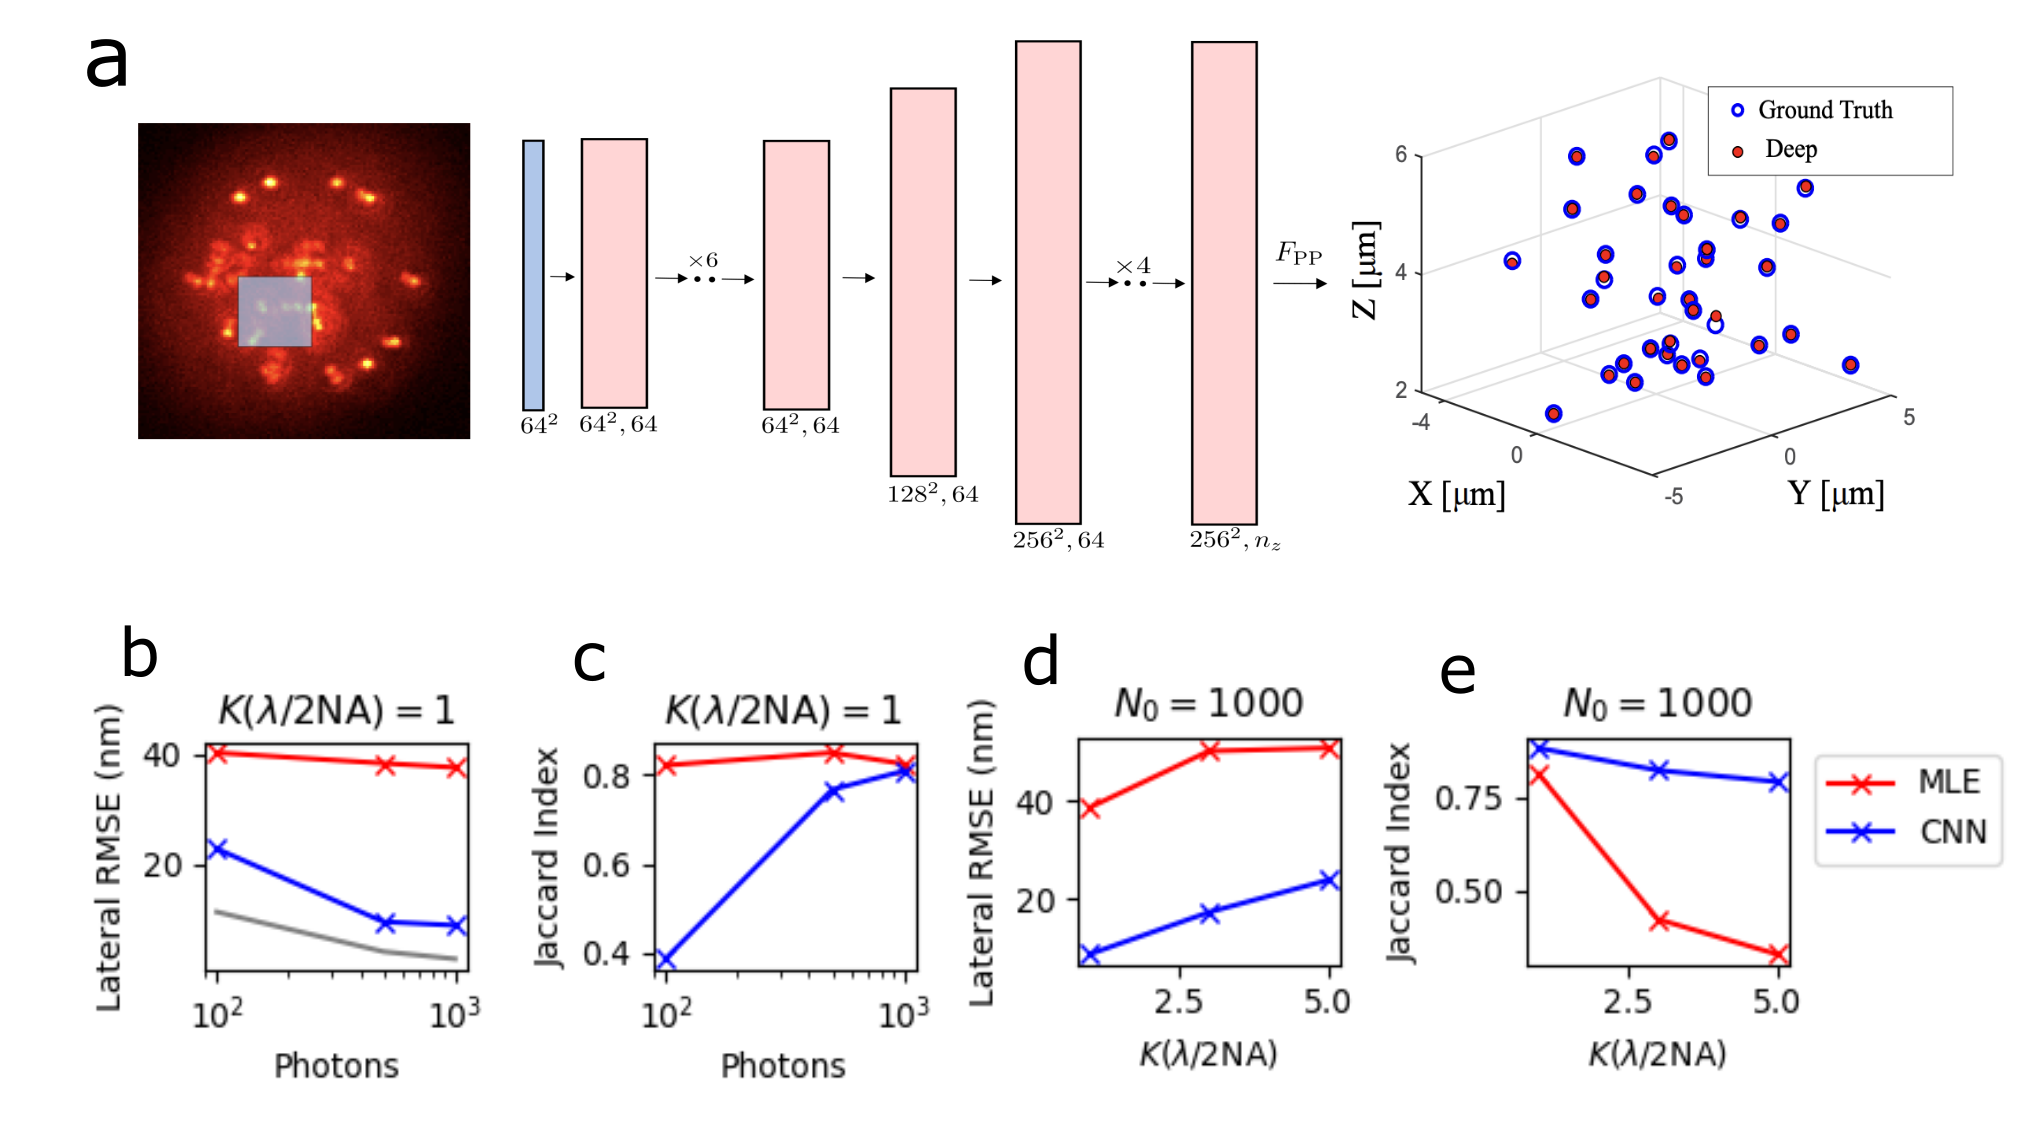
\includegraphics[width=16cm]{PSF2D.png}
\end{center}
\end{figure}

\begin{figure}
\begin{center}
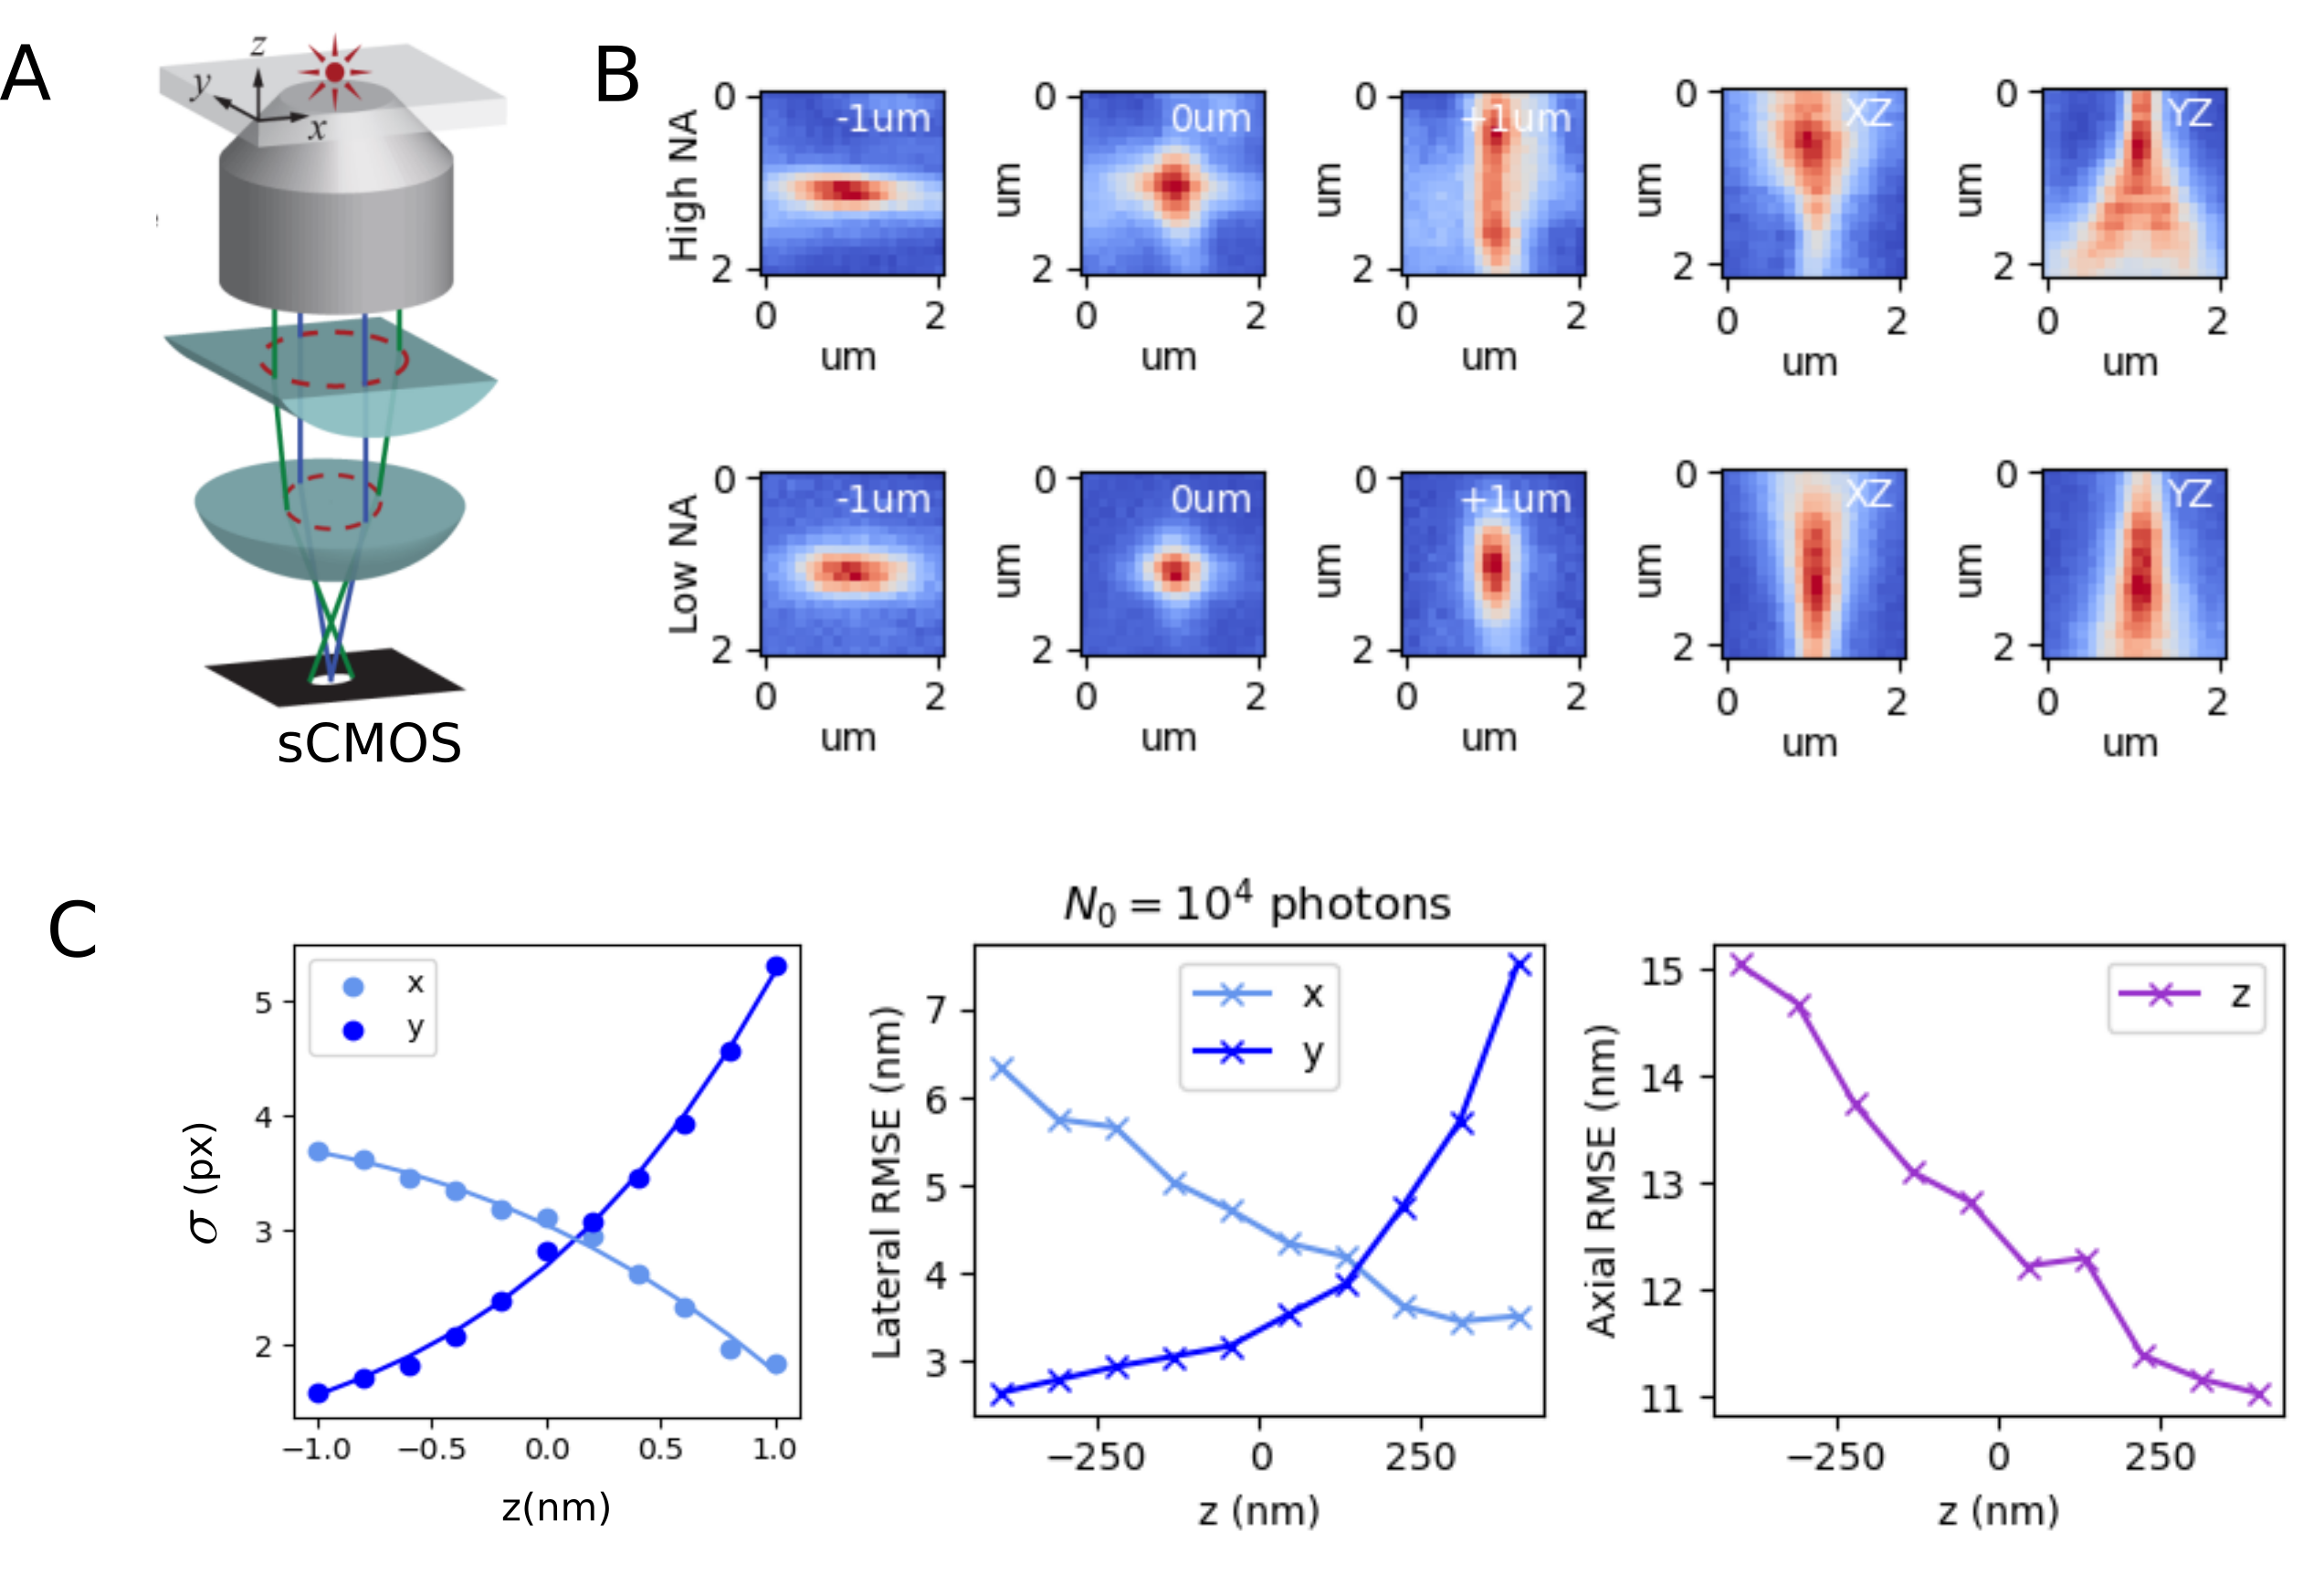
\includegraphics[width=16cm]{Astigmatism.png}
\end{center}
\end{figure}

\section{Visualizing nucleosome cluster dynamics in BRD4 condensates}

For live cell super-resolution of chromatin nanodomains, the HaloTag fusion protein and its associated JF549-HaloTag and JF646-HaloTag ligands have surfaced as indispensable tools (Grimm 2015). H2B is a suitable choice, since it is one of the histones with fewer tail modifications and functional variants with known function (Kamakaka 2005).

Super-resolved nucleosome organization has been studied extensively in various epigenomic states to reveal segregated nanoclusters, dispersed nanodomains, and compact large aggregates  8–10 . Nucleosomes assemble into heterogeneous clusters of variable sizes, interspersed with nucleosome-depleted regions (Ricci 2015). Histone modifications regulate the packaging of nucleosomes into a higher-order chromatin structure to influence the accessibility of genomic DNA to transcription machinery. Higher-order chromatin structure is implicated in a number of cellular processes including gene regulation (Hnisz 2017; Sabari 2018; Boija 2018), DNA damage and repair (Locatelli 2022), as well as cell differentiation and immune activation (Lin 2022). However, identification of key determinants of nucleosome organization at super-resolution remains limited by a lack of live cell and high frame-rate SMLM techniques. Direct visualization of dynamic nucleosome organization over a time scale of hours could provide new insights into the role of higher order chromatin organization in a variety of cellular functions.  

Here, we provide an approach to fast reconstruction of nucleosome organization in living cells. Previous approaches to live cell imaging of chromatin nanodomains only provide ensemble snapshots of chromatin structure due to slow acquisition times (Nozaki 2017). By leveraging the long dark state lifetime of JF646 at moderate laser power, we reconstruct a map of H2B organization in living Hela cells, without sacrificing considerable resolution. Resolution in SMLM is more nuanced and scales with the signal to noise ratio (SNR) and the geometry of the underlying biological structure. Therefore, we develop an image formation model which accounts for sCMOS noise characteristics, molecular density as measured with Ripley’s K-function (Ripley 1977), and a two-state photoswitching model. The sCMOS camera architecture results in every pixel having a unique noise characteristic, and the noise variances of individual pixels can reach thousands of analog-to-digital units squared (Huang 2013). This localization problem is exacerbated in dense scenarios where localization precision and detection accuracy diminish for high duty cycle photoswitching, resulting in significant deviations from the Cramer-Rao lower bound (Speiser 2021). We circumvent these challenges by combining high duty cycle dSTORM with a convolutional neural network (CNN) architecture for fast and accurate single molecule localization (Speiser 2021, Nehme 2020). 

To visualize dynamics of nucleosome organization in interphase nuclei, we recorded dSTORM time-series using oblique illumination microscopy to illuminate a thin area within a single nucleus (Tokunga 2008; Nozaki 2017). By leveraging high duty cycle SMLM and model-based localization algorithms, we efficiently utilize the photon budget and capture super-resolution movies of HaloTag-H2B over long time scales. Our approach complements the short lifetime non-fluorescent state of a HaloTag ligand in a reducing environment with a localization algorithm trained on simulated dense SMLM time-series (iterative Richardson-Lucy deconvolution with the point spread function and maximum likelihood fitting). The method is extended further by two-color labeling to reveal the respective partitions of fast and slow-diffusing H2B in relation to the structure of chromatin nanodomains.  


\begin{figure}
\begin{center}
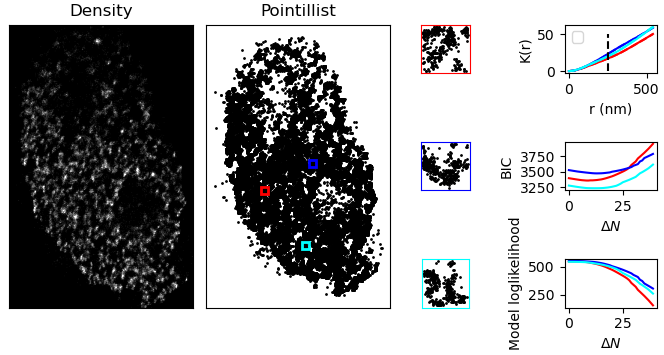
\includegraphics[width=16cm]{Cluster.png}
\end{center}
\end{figure}


\end{document}


